\subsubsection{Architecture}
\begin{itemize}
    \item 60 cores, In-order\cite{phi_specs}.
    \item 1.053 GHz of clock speed per core\cite{phi_specs}.
    \item Every core contains a 512-bit vector arithmetic unit(executing SIMD vector instructions). It fits 8 double precision 
        floating point numbers, or 16 single precision floating point numbers. Each core can issue a single vector instruction per
        cycle\cite{opencl_phi}, so vector instructions issued by different threads in the same core are sequentialized, they do 
        not execute in parallel(at the same cycle).
    \item Each core has a L1 cache memory of 32KB for data and 32KB for instructions(64KB total). Miss latency 15-30
        cycles and access to L1 cache has a latency of 1 cycle\cite{opencl_phi}.
    \item Each core has a L2 cache of 512KB between data and instructions(combined 30MB of L2 cache). Miss latency 500-1000 cycles
        \cite{opencl_phi,phi_specs}.
    \item High speed interconect between L2 caches and the memory subsystem\cite{opencl_phi}.
    \item Each core can execute 4 hardware threads simultaneously, 240 threads in total. These threads help to hide 
        instruction and memory latency\cite{opencl_phi}.
\end{itemize}

\par{OpenCL hides most of this detail from the programmer, figure \ref{PhiArch} shows a global view of the Intel Xeon Phi 
    architecture.\cite{opencl_phi}}

\begin{figure}[!h]
    \centering
    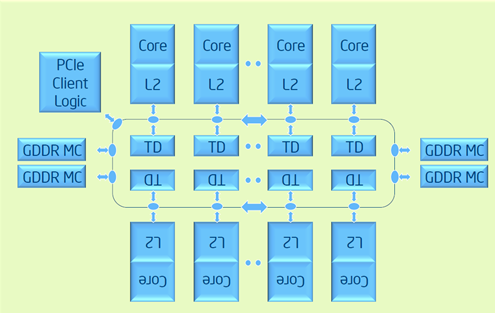
\includegraphics[width=0.6\textwidth]{figures/phi_arch.png}
    \caption{Intel Xeon Phi architecture\cite{opencl_phi}.}
    \label{PhiArch}
\end{figure}


